\chapter{Fault  Analysis }
\textit{In this chapter, probable faults in the system are examined using a  Failure Mode and Effects Analysis (FMEA). Next, in order to find how probable a fault will happen and the effect of it, the severity and occurrance (SO)  of faults is analyzed. It was decided that the fault analysis will be carry out only for the actuators (magnetorquers and momentum wheels).}

\nomenclature[A]{\textbf{FMEA}}{Failure Mode and Effects Analysis}
\nomenclature[A]{\textbf{SO}}{Severity and Occurrance}
\nomenclature[A]{\textbf{FDI}}{Fault Detection and Isolation}
\nomenclature[S]{$\vec{{F}_{MT}}$}{The fault vector for the magnetorqers}
\nomenclature[S]{$\vec{{F}_{RW}}$}{The fault vector for the reaction wheels}

A fault in a system can be seen as a sudden shift in the system functionality, nevertheless, it might not mean a total shutdown of the system. One way to see it is as a disturbance in the system, that might cause performance loss or serious deterioration to the system. On the other hand, a failure can be understood as a total shutdown of the system component. 

In \figref{fig:1} a fault tolerant system is shown, which contains an autonomous supervisor that has the ability to switch between various controllers taking into account the type of fault that a component has. The spacecraft block illustrated in the picture is composed of a plant, actuators and sensors and is monitored by the fault detection and isolation  (FDI) system, which include detectors that will feed informations to the supervisor in the eventuality of a fault. Based on the information received, the supervisor will establish if a fault occurred or not and in case of a fault the effectors will handle it. Figure \ref{fig:2} shows the procedure of how faults are handled with varius methods. The first step in Fault Analysis is fault modelling which uses a procedure called FMEA.
\begin{table}[H]
	\begin{minipage}[b]{0.49\linewidth}
		\centering
		\begin{figure}[H]
			\centering
			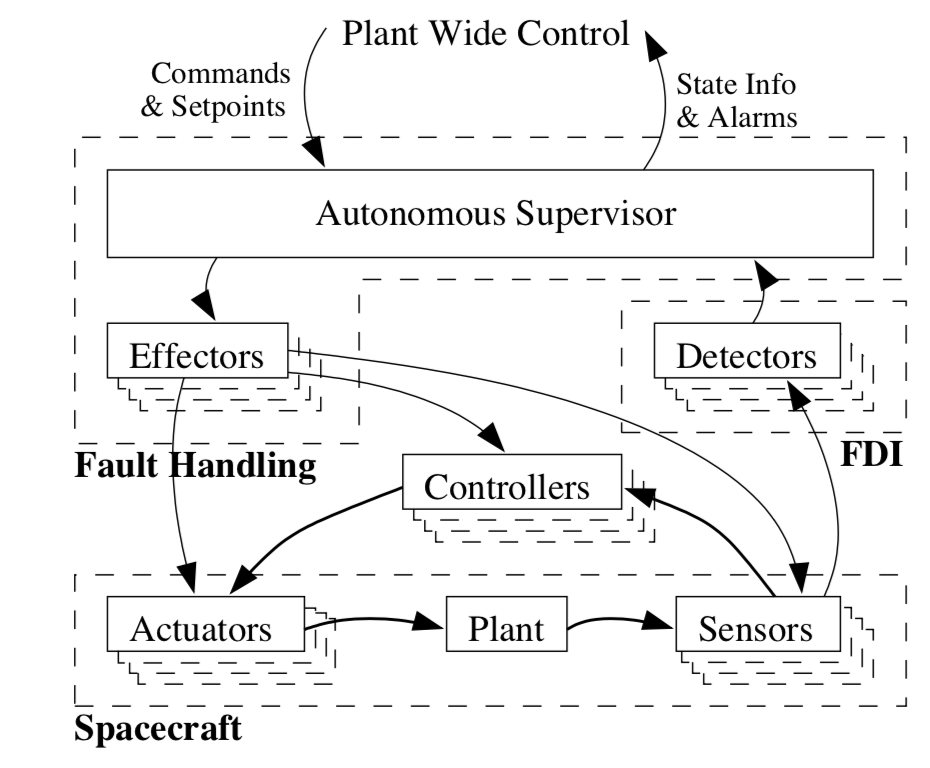
\includegraphics[width=1\linewidth]{figures/FTC}
			\caption{Fault tolerant system architecture \cite{FTJ}}
			\label{fig:1}
		\end{figure}
	\end{minipage}\hfill
	\begin{minipage}[b]{0.49\linewidth}
		\centering
		\begin{figure}[H]
			\centering
			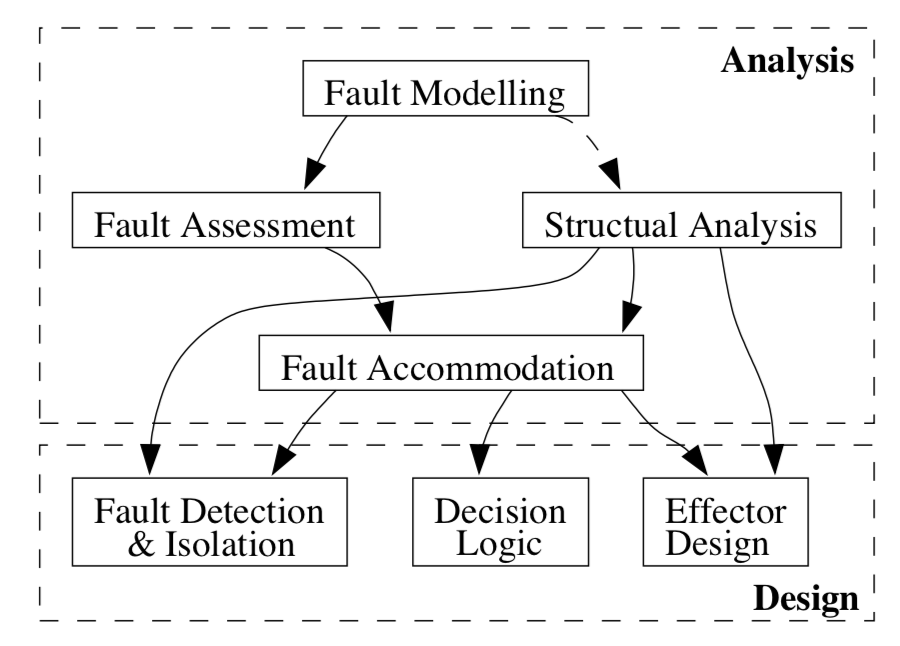
\includegraphics[width=1\linewidth]{figures/FTC_2}
			\caption{ }
			\label{fig:2}
		\end{figure}
	\end{minipage}
\end{table}
\subsection{Failure Mode and Effects Analysis}

\todo{perhaps simplify }

A FMEA analysis which is a bottom-up analysis method is performed for the components of the satellite. The main goal of FMEA is to identify possible faults and their effects on components. In order to evaluate how faults are propagated through the system, a FMEA scheme is constructed.
Another aspect of FMEA analysis is that, the severity of a fault can be determined, which will offer the opportunity to prioritize the faults by severity and in this way focus on the important faults.

In order to control the attitude of the satellite, two types of actuators are used: magnetorquers and reaction wheels. Potential faults are gather into a table which describes the effect and cause, while the satellite is orbiting.
\subsubsection{Magnetorquers}
\begin{table}[H]
	\centering
	\label{my-label}
	\begin{tabular}{|l|l|l|}
		\hline
		\multicolumn{3}{|c|}{\textit{\textbf{Magnetorquers}}}                                          \\ \hline
		\multicolumn{3}{|c|}{Creates a magnetic field that interacts with Earth's magnetic field}                     \\ \hline
		\textbf{Reference} & \textbf{Failure Effect} & \textbf{Failure Cause}                          \\ \hline
		$MT1$                 & Low magnetic field  & \begin{tabular}[c]{@{}l@{}}1) Broken wire or bad soldering\\ 2) Component burned\end{tabular} \\ \hline
		$MT2$                 & Maximum magnetic field power  & Short circuit to the power voltage   \\ \hline
		$MT3$                 & Wrong direction of the magnetic field & \begin{tabular}[c]{@{}l@{}} 1) Misalignment of the magnetorquer\\ 2) Short circuit of some parts of the \\ torquer to the power voltage \end{tabular} \\ \hline
		$MT4$                 & Wrong  power of the magnetic field                 & Floating supplay voltage                                            \\ \hline
	\end{tabular}
	\caption{Potential faults in the magnetorquers}
\end{table}
Description of faults in the magnetorquers: 

$\mathcal{F}_{MT1}$: 
The coil it might have a broken wire or a bad soldering inside, that will lead to a poor generation of magnetic field from the magnetorqers. On the other hand, a component could be burned due to a fluctuation in the current. \todo{voltage regulator is the reason}

$\mathcal{F}_{MT2}$: 
With a short circuit in the power supply, a maximum magnetic field power is expected.

$\mathcal{F}_{MT3}$:
A misalignment of the magnetorquer  due to transportation or a sudden shift during the launch, could affect the direction of the magnetic field.

$\mathcal{F}_{MT4}$:  
A variable supply voltage that could mean a positive or negative operation will end up with an error power of the magnetic field.

The fault vector for the magnetorqers is constructed as follows:

$\mathcal {\vec{{F}_{MT}}}$ = [ \ $\mathcal{F}_{MT1}$ \ $\mathcal{F}_{MT2}$ \ $\mathcal{F}_{MT3}$ \ $\mathcal{F}_{MT4}$ ]$^ \mathsf{T}$
\subsubsection{Reaction wheels}
\begin{table}[H]
	\centering
	\label{my-label}
	\begin{tabular}{|l|l|l|}
		\hline
		\multicolumn{3}{|c|}{\textit{\textbf{Reaction wheels}}}                                          \\ \hline
		\multicolumn{3}{|c|}{Produces a torque about the satellite COM in order to rotate it }                     \\ \hline
		\textbf{Reference} & \textbf{Failure Effect} & \textbf{Failure Cause}                          \\ \hline
		$RW1$                & Faulty orientation & \begin{tabular}[c]{@{}l@{}} Shifting of the flywheel  \\   \end{tabular} \\ \hline
		$RW2$                & Unable to control the rotation   & A short-circuit in the power supply  \\ \hline
		$RW3$                & Low power received& \begin{tabular}[c]{@{}l@{}} Short circuit to the ground\\  \end{tabular} \\ \hline
		$RW4$                & No torque received  &  A fault in windings    \\ \hline
	\end{tabular}
	\caption{Potential faults in the reaction wheels}
\end{table}
Description of faults in the reaction wheels: 

$\mathcal{F}_{RW1}$: 
A displacement of the flywheel throughout launch or transportation could result in a error in the orientation that might alter the angular velocity of the satellite.

$\mathcal{F}_{RW2}$: 
A short-circuit in the power supply could influence the rotation of the flywheel, by having a low or maximum rotation, which will end up with a low or maximum power.

$\mathcal{F}_{RW3}$:
A short circuit to the ground due to a borken wire or bad soldering will result in low power generation, that could influence the rotation of the flywheel.

$\mathcal{F}_{RW4}$:  
Due to a fault in the windings, the flywheel will not be able to rotate, therefore, no torque will be received.

The fault vector for the reaction wheels is constructed as follows:

$\mathcal {\vec{{F}_{RW}}}$ = [ \ $\mathcal{F}_{RW1}$ \ $\mathcal{F}_{RW2}$ \ $\mathcal{F}_{RW3}$ \ $\mathcal{F}_{RW4}$ ]$^ \mathsf{T}$
\subsubsection{Severity and occurrence evaluation}
The next step into Fault Analysis is the Fault Assessment that involves a Severity Occurrence analysis
To investigate the faults that have the biggest rate of occurrence, the severity of the effects of failures and the probability of occurrence is determined based on the faults from FMEA. This procedure describes how to each fault receives a severity index \nomenclature[A]{\textbf{SI}}{Severity Index} (SI) and an occurrence index \nomenclature[A]{\textbf{OI}}{Occurrence Index} (OI). A table containing the serverity and occurrence for magnetorquers is shown as follows:
\begin{table}[H]
	\centering
	\label{11}
	\begin{tabular}{|l|l|l|l|}
		\hline
		\multicolumn{4}{|c|}{\textit{Magnetorquer}}                                                                                         \\ \hline
		Reference & Severity & Occurrence                                          & SO Index                                      \\ \hline
		$MT1$     & 7        & \begin{tabular}[c]{@{}l@{}} 5\\  4\end{tabular} & \begin{tabular}[c]{@{}l@{}} 35\\ 28\end{tabular} \\ \hline
		$MT2$       & 10       & 3       & 30                \\ \hline
		$MT3$       & 3        & \begin{tabular}[c]{@{}l@{}}2\\ 1\end{tabular} & \begin{tabular}[c]{@{}l@{}}6\\ 3\end{tabular} \\ \hline
		$MT4$       & 4        & 6                   & 24                  \\ \hline
	\end{tabular}
\caption{SO for magnetorquer}
\end{table}
The same procedure is done for momentum wheels as follows:
\begin{table}[H]
	\centering
	\label{12}
	\begin{tabular}{|l|l|l|l|}
		\hline
		\multicolumn{4}{|c|}{\textit{Reaction wheels}}                                                                                         \\ \hline
		Reference & Severity & Occurrence                                          & SO Index                                      \\ \hline
		$RW1$      & 1        & \begin{tabular}[c]{@{}l@{}}7\\ \end{tabular} & \begin{tabular}[c]{@{}l@{}}7\\ \end{tabular} \\ \hline
		$RW2$        & 1        & 4             & 4                                         \\ \hline
		$RW3$        & 2        & \begin{tabular}[c]{@{}l@{}}3\\\end{tabular} & \begin{tabular}[c]{@{}l@{}}8\\ \end{tabular} \\ \hline
		$RW4$        & 4        & 2     & 8               \\ \hline
	\end{tabular}
	\caption{SO for momentum wheels}
\end{table}

The severity index is computed using the following formula:
\begin{flalign}
	SO_{index} = severity \cdot occurrence
	\label{eq:ec1}
\end{flalign} 

%\subsubsection{Fault propagation analysis}
%In order to observe how faults are propagated through the system and the effect of these faults, a FMEA scheme is constructed. Further computation will be on the appendix.
